% CREATED BY DAVID FRISK, 2016
\chapter{Theory}


\section{Krug's theory: What is usability, and how do you test it?}

Steve Krug is a usability consultant who wrote books about usability. His usability books are mainly focused on websites, but as he writes himself, his methods are applicable on other things as well.

Krug defines his first law of usability as "Don't make me think!", implying that users should be understand what a website is and how to use it without expending any effort thinking about it:

"A person of average (or even below average) ability and experience can figure out how to use the thing to accomplish something without it being more trouble than it's worth." [SOURCE: DON'T MAKE ME THINK REVISITED, p.9]

Aside from a few principles of usability, Krug puts a lot of effort into describing the usefulness of usability testing and how to do such testing in a cheap and easy manner. In his book specifically about usability testing, he defines such tests as:

"Watching people try to use what you're creating/designing/building (or something you've already created/desgined/built), with the intention of (a) making it easier for people to use or (b) proving that it is easy to use."

Or, in simpler terms:

"A facilitator sits in a room with the participant, gives him some tasks to do, and asks him to think out loud while he does them."

\subsection{Making usability testing scientific}

One important difference between Krug's method and the method used in this thesis is that Krug's focus is not tobe scientific, but to merely improve what one is building [SOURCE: ROCKET SURGERY MADE EASY]. Thus, certain parts of his method have been adapted to make it easier to analyze:

\begin{enumerate}
	\item In contrast to Krug's method, the tasks in the tests are not altered mid-test, to make them more comparable.
	\item There is more data gathering involved in the form of recordings and notes, rather than having a group of observers watching the test, to make analysis and comparison easier long after the tests have been conducted.
\end{enumerate}

\subsection{Connecting usability theory for websites to teaching materials}

One can argue that there's a large difference between teaching materials and websites. While in some cases these can be the same, such as online materials shared through a blog post, a teaching material can sometimes take the form of a book, a single PDF file, and more. All the materials have in common is that they're used to facilitate and/or empower a teacher's work. However, usability testing is still clearly applicable in the sense that it consists of observing someone use what you're testing.

Since teaching materials can be used in many different ways, the use case had to be narrowed down. Thus, in this thesis, the use case that the usability tests cover consist mainly of how teachers use teaching materials to plan their lessons. This does not mean that other use cases are ignored, such as a teacher simply using a material to learn more about a subject. However, the lesson planning is the main focus of the usability testing in this thesis.

% ----
% In the following sections, examples of a figure, an equation, a table, a chemical structure, a list, a listing and a to-do note are shown.

\section{Figure}
\begin{figure}[H]
\centering
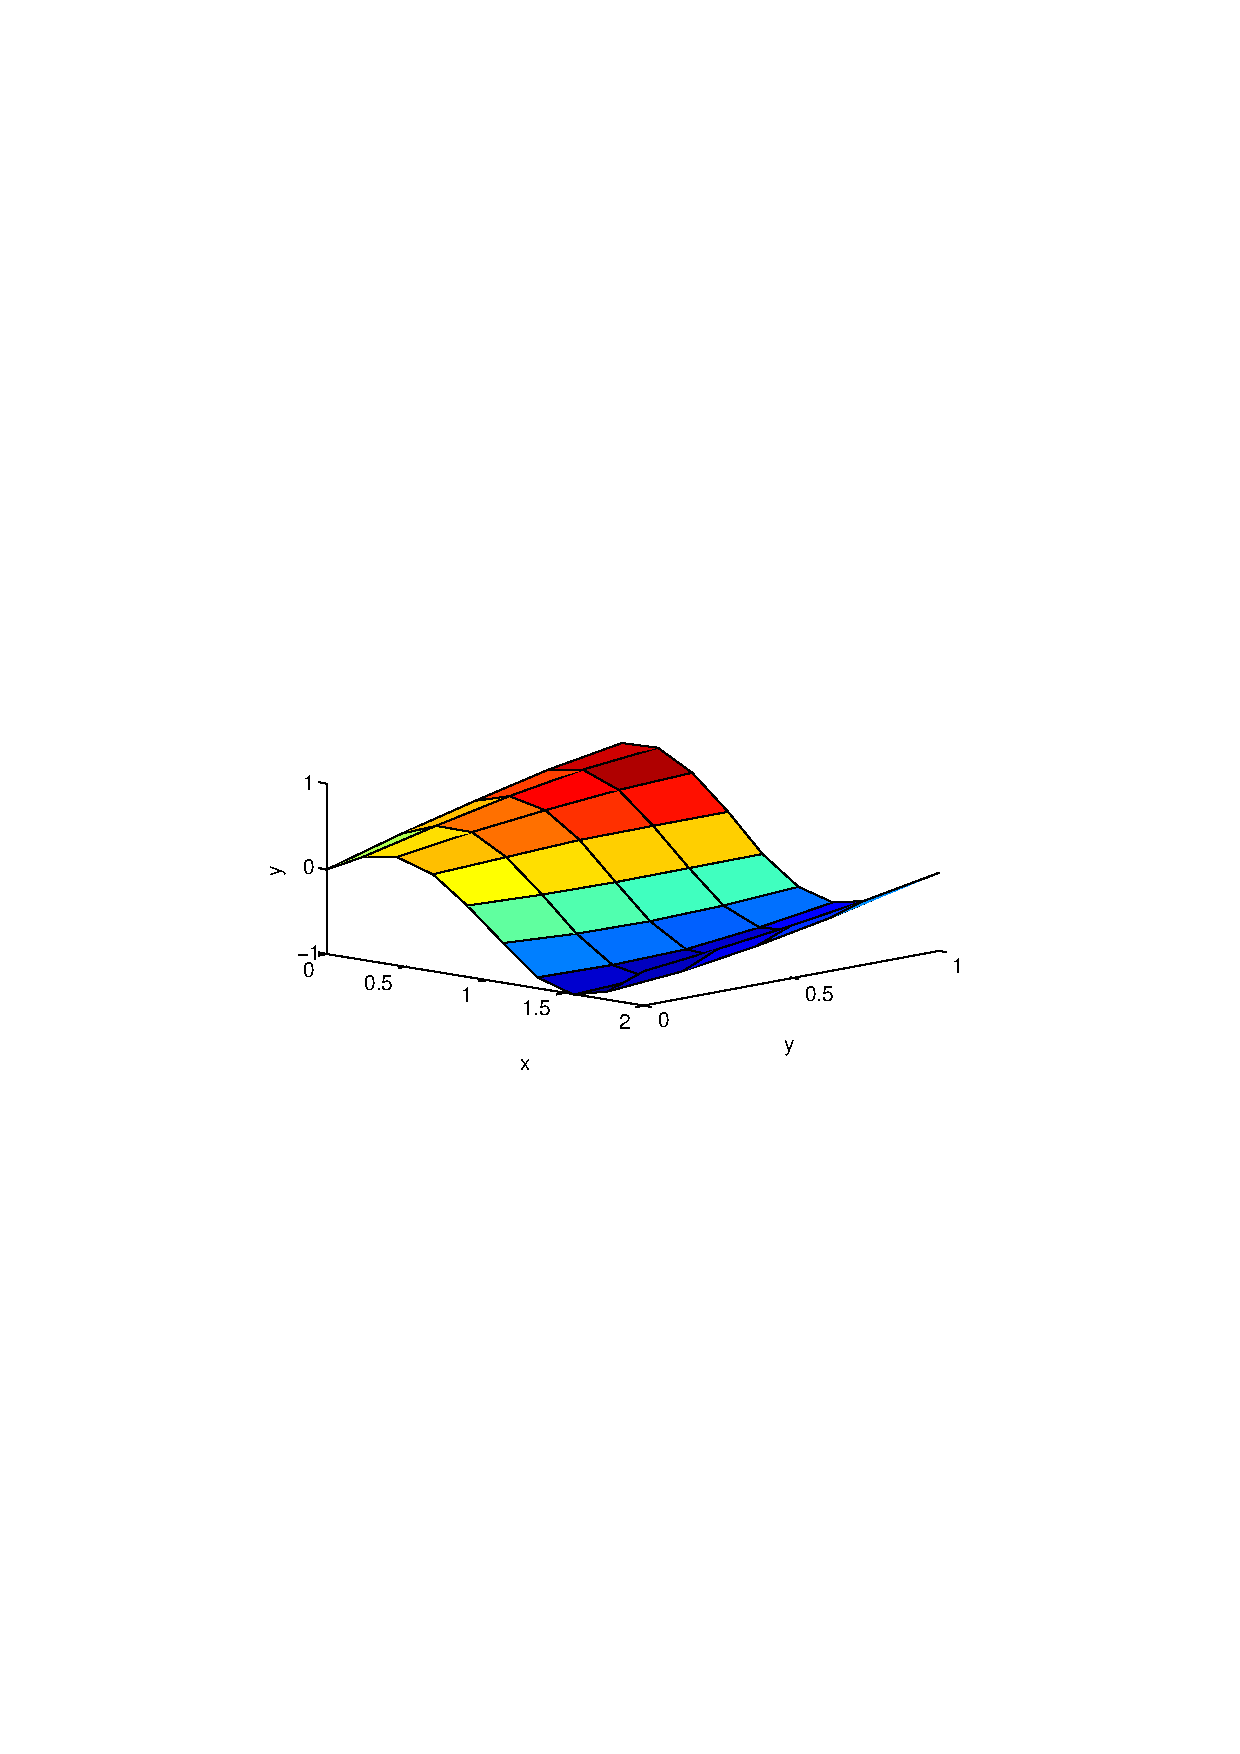
\includegraphics[width=0.45\linewidth, trim=3cm 11cm 3cm 11cm]{figure/X.pdf}
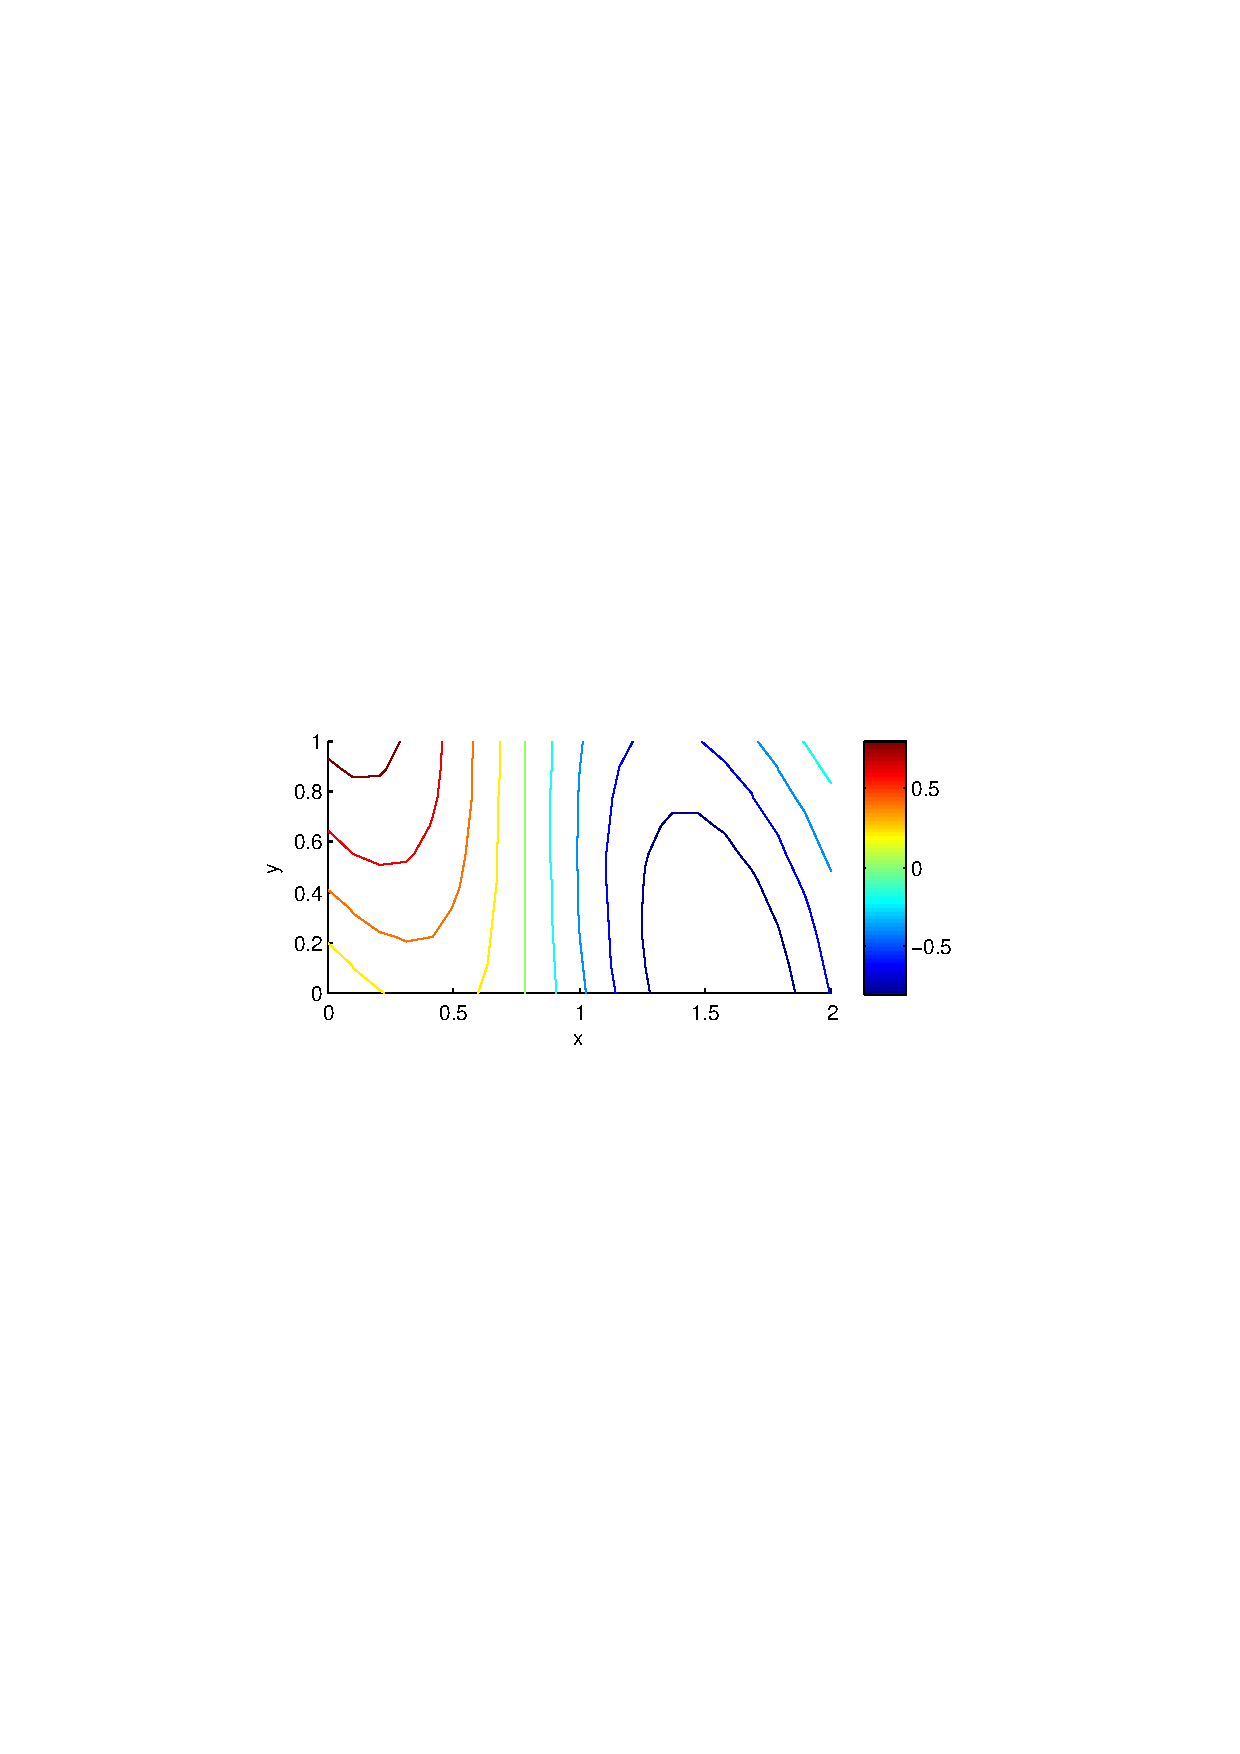
\includegraphics[width=0.45\linewidth, trim=3cm 11cm 3cm 11cm]{figure/Y.pdf}
\caption{Surface and contour plots showing the two dimensional function $z(x,y)=\sin(x+y)\cos(2x)$.}
\end{figure}

\section{Equation}
\begin{equation}
f(t)=\left\{ \begin{array}{ll}
1,~~~~ & t< 1 \\
t^2 & t\geq 1
\end{array}\right.
\end{equation}

\section{Table}
\begin{table}[H]
\centering
\caption{Values of $f(t)$ for $t=0,1,\dots 5$.}
\begin{tabular}{l|llllll} \hline\hline
$t$ & 0 & 1 & 2 & 3 & 4 & 5 \\ \hline
$f(t)$ & 1 & 1 & 4 & 9 & 16 & 25 \\ \hline\hline
\end{tabular}
\end{table}

\section{Chemical structure}
\begin{center}
\chemfig{X*5(-E-T-A-L-)}
\end{center}

\section{List}
\begin{enumerate}
  \item The first item
  \begin{enumerate}
    \item Nested item 1
    \item Nested item 2
  \end{enumerate}
  \item The second item
  \item The third item 
  \item \dots
\end{enumerate}

\section{Source code listing}
%\lstset{language=Matlab}
\begin{lstlisting}[frame=single]
% Generate x- and y-nodes
x=linspace(0,1); y=linspace(0,1);

% Calculate z=f(x,y)
for i=1:length(x)
 for j=1:length(y)
  z(i,j)=x(i)+2*y(j);
 end
end
\end{lstlisting}

\section{To-do note}
The \texttt{todo} package enables to-do notes to be added in the page margin. This can be a very convenient way of making notes in the document during the process of writing. All notes can be hidden by using the option \emph{disable} when loading the package in the settings. \todo{Example of a to-do note.}

